%! Author = brdvlami
%! Date = 30/04/2024

% Preamble
\documentclass[11pt]{article}

% Packages
\usepackage[english]{babel}
\usepackage{subfloat}
\usepackage{float}
\usepackage[style=ieee, backend=biber]{biblatex}
\addbibresource{abstract_bibliography.bib}
\renewcommand*{\bibfont}{\footnotesize}

\usepackage[small]{titlesec}
\titlespacing*{\section}{0pt}{3ex}{1ex}
\titlespacing*{\subsection}{0pt}{3ex}{0.5ex}
\titlespacing*{\subsubsection}{0pt}{3ex}{0.5ex}
\usepackage{multicol}
\usepackage{caption}
\captionsetup{font=footnotesize}
\usepackage[hyperfootnotes=true]{hyperref}
\usepackage{xcolor}
\hypersetup{
    colorlinks,
    linkcolor={black},
    citecolor={blue!50!black},
    urlcolor={blue!80!black}
}
%\setlength{\parindent}{0em}
\usepackage{geometry}
\geometry{
    a4paper,
    left=15mm,
    right=15mm,
    top=15mm,
    bottom=25mm,
}
\usepackage{graphicx}
\graphicspath{{./figures/}}

\newenvironment{Figure}
{\par\medskip\noindent\minipage{\linewidth}}
{\endminipage\par\medskip}


\newenvironment{Table}
{\par\medskip\noindent\minipage{\linewidth}}
{\endminipage\par\medskip}

\babelhyphenation[english]{Uni-Prot-KB}

% Document
\begin{document}

    \begingroup
    \centering
    \LARGE Unipept 6.0: Fast semi-exact peptide matching with a memory conservative index for UniProtKB\\[1em]
    \large Bram Devlaminck\\[2em]
    \endgroup

    \par\noindent\rule{\linewidth}{.5pt}
    \section*{Abstract}\label{sec:test-section}
    Unipept is an ecosystem developed for fast metaproteomics data analysis.
    In the past few years, Unipept has been optimized for tryptic peptide search, with a slow workaround for peptides with missed cleavages.
    Unipept 6.0 introduces a new index structure which allows fast peptide matching for arbitrary peptides.
    This makes Unipept applicable in domains where trypsin is not the protease of choice, and also removes the introduced performance penalty when dealing with missed cleavages.
    In addition to these advancements, Unipept 6.0 maintains its superior performance compared to similar tools, ensuring efficient and accurate metaproteomics data analysis.
    \par\noindent\rule{\linewidth}{.5pt}

    \begin{multicols}{2}
        \section{Introduction}\label{sec:introduction}
        Traditionally, the most used protease in the (meta)proteomics field is trypsin.
        Unipept~\cite{unipept_desktop, unipept_api, unipept_4, unipept_orig, unipept_tutorial, unipept_web, unipept_cli, unipept_desktop_2} was specifically developed with this in mind.
        This resulted in the use of an index structure where the UniProtKB~\cite{UniprotKB} database is preprocessed by splitting every protein according to the cleavage pattern created by trypsin.
        This also allows Unipept to precompute the LCA for every possible combination of matching tryptic peptides.
        This approach has proven its efficiency in the past few years, but also has its limitations.

        From time to time, trypsin will miss a cleavage position.
        This creates a so-called missed cleavage.
        Peptides with such missed cleavages will not be present in the current Unipept index, since Unipept assumes there are no missed cleavages.
        To solve this problem, a solution was retro-fitted to handle these missed cleavages.
        When this option is selected, Unipept will scan the input peptide for these missed cleavage positions, split the peptide and perform separate lookups for every tryptic fragment.
        The resulting sets of matches are intersected, which delivers a set of possible protein matches.
        Every protein in this set is brute-force scanned to ensure that the complete original peptide is present, and not only the separate tryptic fragments.
        Finally, the LCA of the found proteins is calculated on the fly.
        All these extra steps, including the on the fly calculation of the LCA, have a significant impact on the performance.

        A second disadvantage of the current Unipept index is the inability to process non-tryptic peptides.
        Similar to peptides with missed cleavages, these will not be present in the index, but no workaround exists in this case.

        This restriction has not been a significant problem since Unipept was originally created for the metaproteomics field, where trypsin is widely used.
        However, other fields, such as the immunopeptidomics field, frequently work with non-tryptic peptides.
        We aspire to broaden the use cases of Unipept, which requires a new search index with the following properties:

        \begin{enumerate}
            \item For every peptide (tryptic or non-tryptic), all matches in UniProtKB should be found.
            \item The maximum memory usage when building the index for the complete UniProtKB database should be around 1 to 2 TB\@.
            \item Search performance should be on par with the current Unipept tryptic peptide search.
            \item The new index should facilitate all the current Unipept features.
        \end{enumerate}

        In short, we want an index that does not remove any of the current features, while eliminating the restriction that only tryptic peptides can efficiently be found by the current index.
        This also means that our new index will need to provide a way to equalize the amino acids isoleucine and leucine, as this is a core feature.


        \section{Methods}\label{sec:methods}
        At the core of our new index structure is a suffix array.
        This suffix array can be build using the libdivsufsort~\cite{libdivsufsort} or libsais~\cite{libsais} library.
        Both provide a linear time algorithm with a $5n + O(1)$ memory complexity, where $n$ is the size of the text that needs to be indexed.
        Depending on the used text, one is faster than the other.

        \subsection{Sparse Suffix Arrays}
        While a complete suffix array delivers the best performance, the index itself is large.
        The size of the suffix array can be reduced by introducing a sampling step to create a so-called sparse suffix array (SSA).
        This variant of a suffix array only stores every $k$-th suffix of the input text.
        This results in an SSA which is only $\frac{1}{k}$ of the original suffix array size.
        The disadvantage of using an SSA is that it becomes impossible to search for peptides existing out of less than $k$ amino acids, and that searching in general becomes slower.
        This trade-of does not introduce any problem, since Unipept already prevents the search of peptides who consist out of less than 5 amino acids.
        This restriction was introduced to improve the performance, while losing a minimum amount of information since short peptides occur in a lot of proteins.
        Searching such a short peptide would yield an extremely generic functional and taxonomic analysis result, which is not interesting to the user.

        \subsection{Equalizing Isoleucine and Leucine}
        Our solution to treat isoleucine and leucine as equal consists of two parts.
        Firstly, we don't index the original text, but a slightly modified version.
        We replace every occurrence of leucine by isoleucine, which essentially equalizes them during the construction of the suffix array.
        During the search, we perform the same translation on every peptide.
        As a result, we find every match with I and L equalized.
        This search is performed using the original, unmodified text.
        This is important, since the original text is needed in an additional second step when a search has to be performed where I and L are not equalized.

        During this second step, we filter away unwanted matches from the first stage.
        This is achieved by checking every I and L location in the original, unmodified peptide with the matching amino acid in the original, unmodified text.
        A mismatch indicates that I and L were wrongfully equalized.
        Only the I and L locations have to be checked since the suffix array search already ensures that all other characters match in the original text.

        \subsection{Analyses}
        Our solution performs the functional and taxonomic analysis at runtime.
        While it would be advantageous to precompute this, the suffix array and text do not contain enough information to do this.
        This is a trade-off we made during development between maximum memory usage and speed.


        \section{Results}\label{sec:results}
        Three main aspects are considered during testing.
        The memory usage and speed during building, the resulting index size while hosting and search performance.

        \subsection{Building the Index}
        Building the suffix array for the complete UniProtKB database requires around 735 GB of RAM and 5 hours of computing time using the libdivsufsort library.
        Because of the high-memory needs, we use the HPC of Ghent University, where the high-memory cluster has 16 nodes with each 2\times 64-core AMD EPYC 7773X (Milan-X @ 2.2 GHz) and 940 GB of RAM\@.
        We use one core of a single node, since the construction phase is single threaded.
        The resulting full suffix array is around 700 GB large (+ another 88 GB for the text).
        Our goal is to host this new index on Unipept servers, which have around 0.5 TB of available memory.
        To make this possible, we immediately perform a sampling phase with sparseness factor $k = 3$ at the end of the construction process on the HPC\@.
        This results in a search index size of $\frac{700}{3} + 88 \approx 322$ GB\@.
        Next to this search index, Unipept needs extra information (such as the UniProt accession number, NCBI taxon ID and functional annotations per protein) to perform the provided analyses.
        This results in another 25 GB of needed RAM\@.
        Figure~\ref{fig:uniprot_memory_treemap} visualizes the size of each component of the resulting index.

        \begin{Figure}
            \centering
            \resizebox{\textwidth}{!}{
                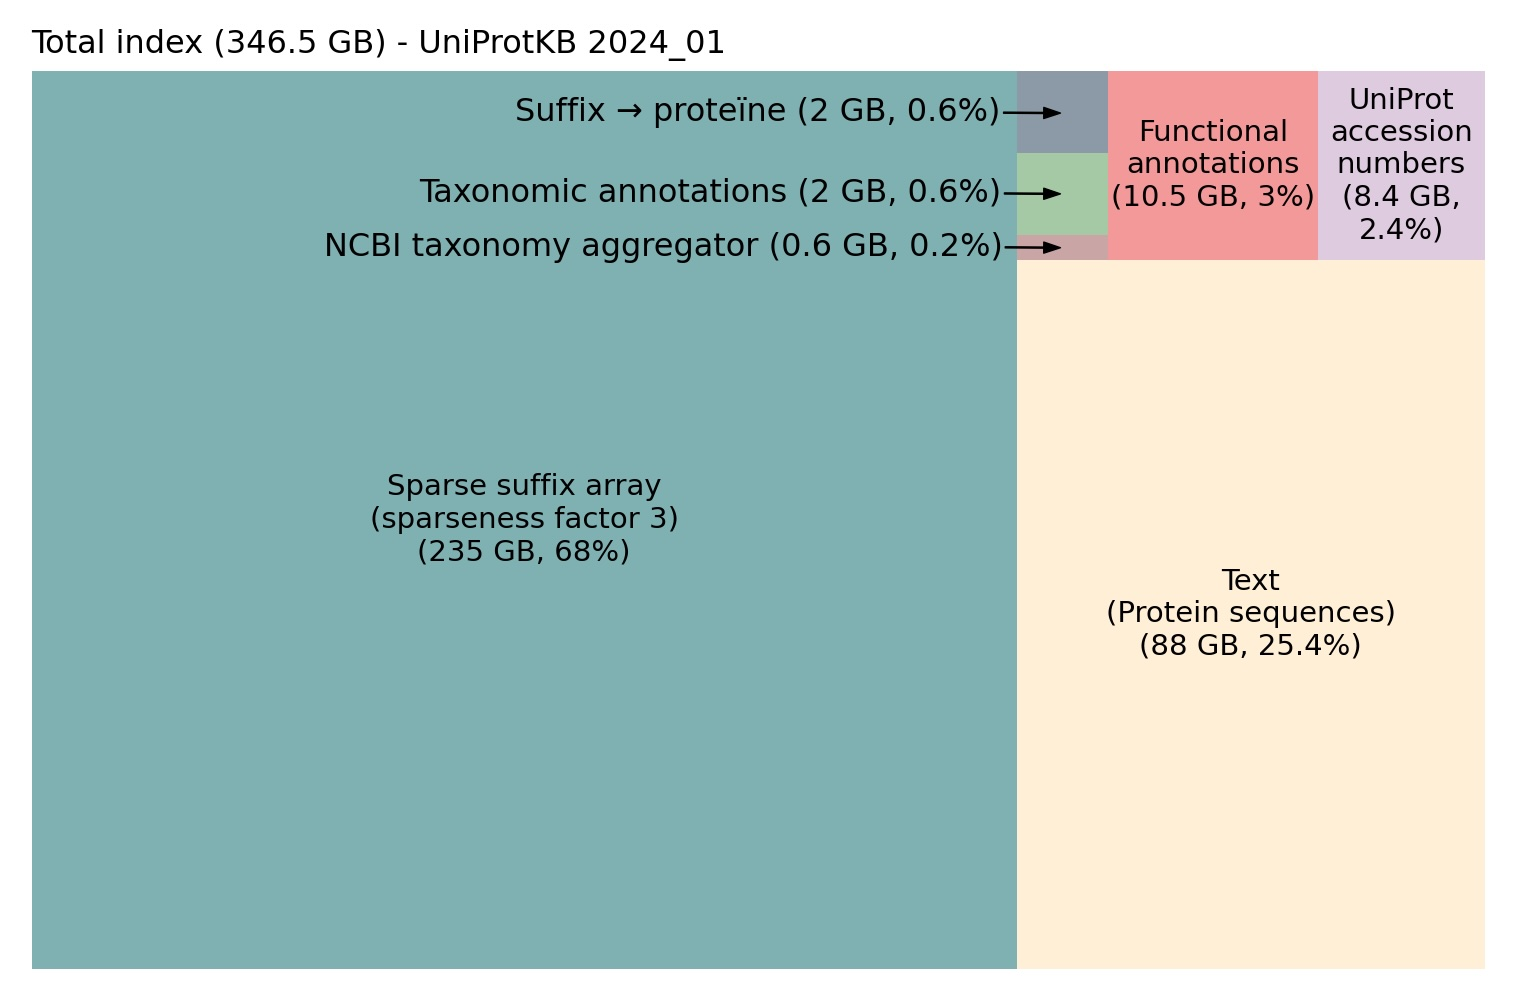
\includegraphics{uniprot_memory_treemap}
            }
            \captionof{figure}{Visualisation of the size of each component of the new Unipept index for UniProtKB 2024\_01.}
            \label{fig:uniprot_memory_treemap}
        \end{Figure}

        \subsection{Querying the Index} % TODO: redo performance timing on new unipept server, or mention this difference
        To evaluate the search performance we use 6 files with each around 25\thinspace000 peptides.
        These are samples from the SIHUMIx experiment~\cite{SIHUMI_frequently_used, SIHUMI_first_introduction}, where trypsin is used as a protease.
        This means that as well as tryptic peptides, there are also peptides present with naturally occurring missed cleavages.
        Figure~\ref{fig:new_vs_old_unipept} shows the execution time for both the new and old unipept index.
        To make the comparison as fair as possible, the \textit{filter duplicate peptides} setting is turned off, and \textit{advanced missed cleavage handling} is turned on.
        This ensures that both the old and new index search every peptide from the input file (including duplicates and peptides with missed cleavages).
        The new index is 10 to 100 times faster, which clearly removes the performance penalty that was currently associated with handling missed cleavages.
        Note that the old Unipept index will not find peptides created by a different protease, while this makes no difference for the new index.
        \begin{Figure}
            \centering
            \resizebox{\textwidth}{!}{
                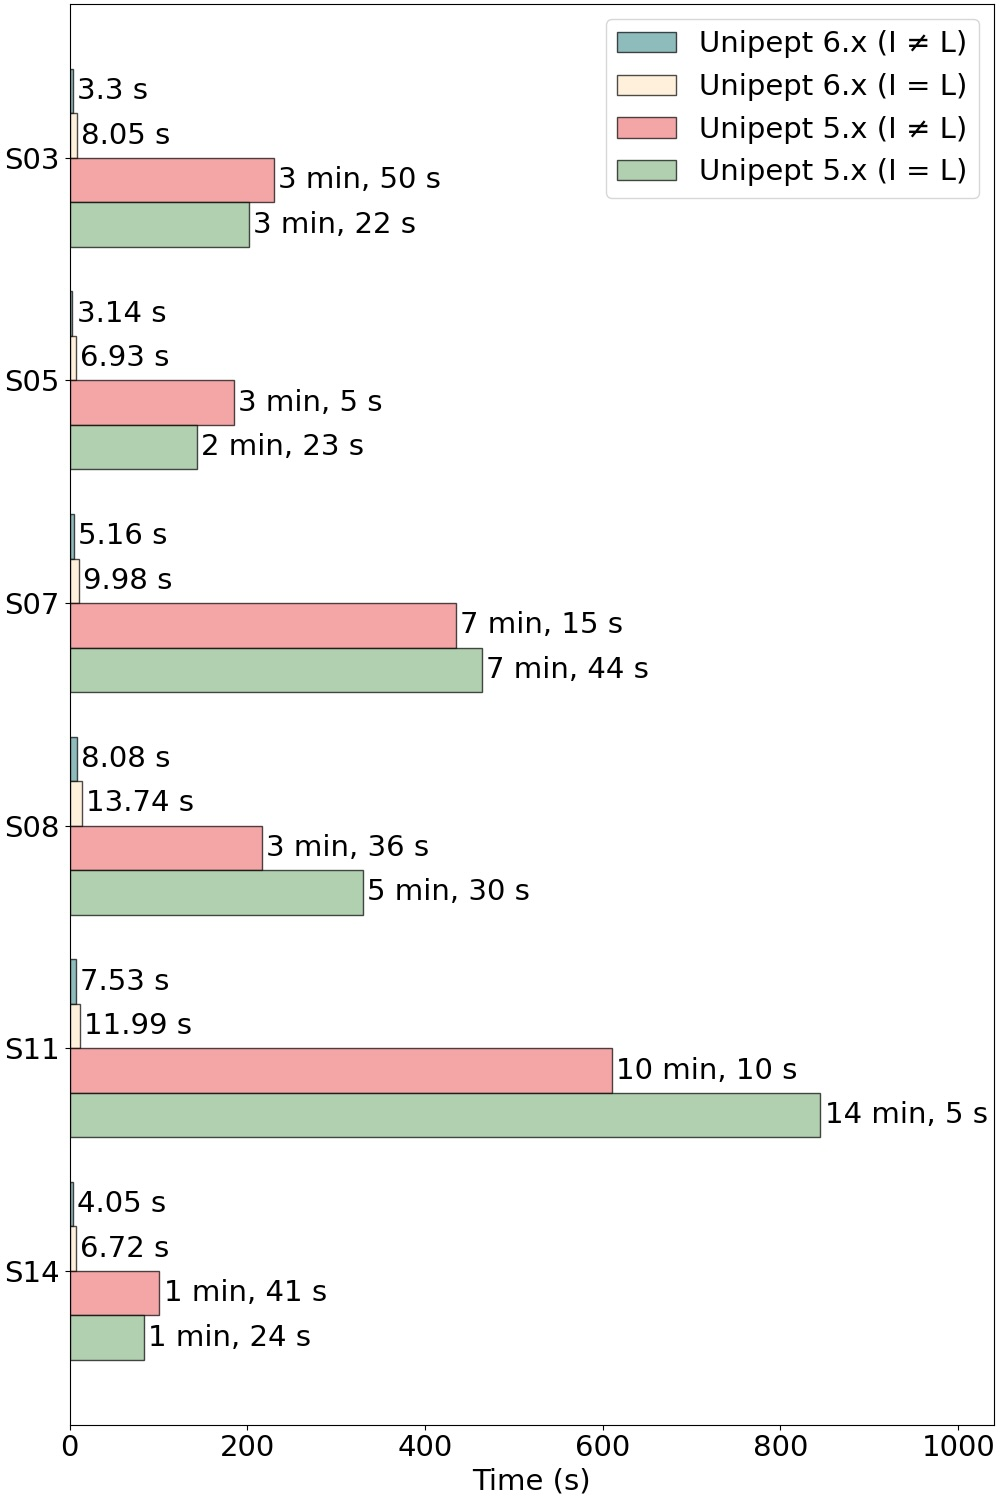
\includegraphics{new_vs_old_unipept}
            }
            \captionof{figure}{Execution time for the new and old Unipept index while searching different SIHUMIx samples. Each sample consists of approximately 25\thinspace000 peptides. The old Unipept index searches with the \textit{filter duplicate peptides} setting turned off, and \textit{advanced missed cleavage handling} turned on. This way both indices search all peptides (included duplicates), and missed cleavages are handled by both. The used test files can be found back in our GitHub repository \url{https://github.com/BramDevlaminck/Thesis_benchmarkdata/tree/master/SIHUMI}}
            \label{fig:new_vs_old_unipept}
        \end{Figure}

        Another interesting case to consider is when searching strictly tryptic peptides.
        This that case, missed cleavage handling can be disabled on the old index, which significantly improves the performance.
        Figure~\ref{fig:new_vs_old_unipept_tryptic} visualizes the search time for 100\thinspace000 tryptic peptides.
        It is visible that the performance is comparable when I and L are equalized, while the old index is around a third faster than the new index when I and L are not equalized.

        Furthermore, it is clearly visible that the extra filtering step, when I $\neq$ L, has a performance impact in the new index.
        This effect was not visible in Figure~\ref{fig:new_vs_old_unipept}, where the reverse seems to be visible.
        However, this reverse effect can be explained by the fact that searching with I = L finds more matches, which requires more output to be serialized to a JSON file.
        When searching for larger files, there is proportionally more time spend in the search phase, which compensates for the longer serialization time.

        \begin{Figure}
            \centering
            \resizebox{\textwidth}{!}{
                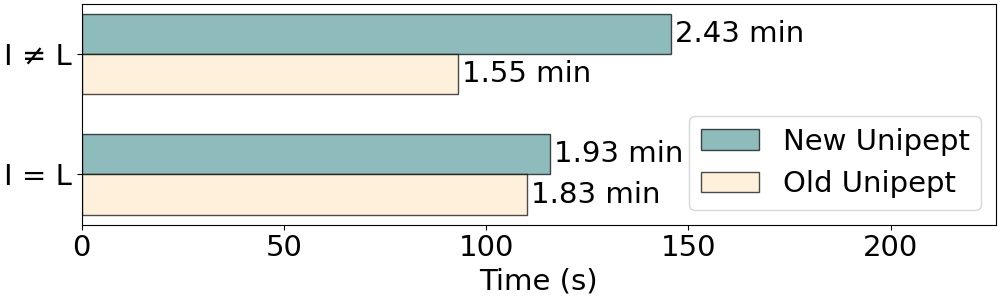
\includegraphics{new_vs_old_unipept_tryptic}
            }
            \captionof{figure}{Search time for 100\thinspace000 tryptic peptides for the new and old Unipept index. This is the best case scenario for the old index where missed cleavages are \textbf{not} handled.}
            \label{fig:new_vs_old_unipept_tryptic}
        \end{Figure}


        \section{Comparison}\label{sec:comparison}
        Tools such as the Uniprot peptide search tool~\cite{uniprot_search_site, uniprot_search_paper}, the Expasy ScanProsite tool~\cite{scanprosite} and the current Unipept release all have the possibility to find matches in the UniProtKB database.
        Next to the performance, we also compare the provided features.
        Because of the limited performance of some tools, we limited testing to the randomly chosen peptide \texttt{ISPAVLFVIVILAVLFFISGLLHLLVR}.
        The new suffix array uses the above described settings and finds all matches for our test peptide in less than 5 ms.

        Feature wise, the UniProt Peptide Search tool is identical to the new suffix array index developed for Unipept.
        They both find all matches in UniProtKB, and have the option to equalize I and L\@.
        The only difference is in the performance.
        Searching our test peptide in the SA only takes a few milliseconds, while the UniProt tool takes a few seconds up to multiple minutes.

        The Expasy ScanProsite tool takes another approach.
        They provide a wide range of options for inexact matching.
        They call this motives, and these are comparable to regular expressions where the user can use wildcards, character classes and even negations.
        The other major difference is that this tool does not use the whole UniProtKB database.
        Only the proteins that are part of a reference genome are indexed, which means only around one third of the complete UniProtKB database is indexed.
        Lastly, searching our test peptide takes around 5 minutes.
        As expected, since not the whole UniProtKB database is index, only a subset of the matches is found.

        The last major tool we compare with, is the current Unipept index.
        The new Unipept index is feature wise identical to the current index, with the addition of removing the restriction where Unipept can only quickly find tryptic peptides.
        This means that every non-tryptic peptide will result in 0 matches in the current index, while the new index will find all matches that are in UniProtKB\@.
        Searching our test peptide took less than 5 ms, and found the same matches because our test peptide is tryptic.
        It is important to note though, if we had chosen a non-tryptic peptide we would not have found any matches.
        Table~\ref{tab:tool_comparison} gives an overview of the described differences between the tools.

        \begin{Table}
            \centering
            \resizebox{\textwidth}{!}{
                \begin{tabular}{ l l l l l }
                    & SSA      & UPS          & ESP        & UP             \\
                    \hline\hline
                    Used proteins    & all      & all          & ref. prot. & all            \\
                    Approx. match    & [IL]     & [IL]         & flexible   & [IL]           \\
                    Time             & $<$ 5 ms & 1 s - 20 min & 5 min      & $<$ 5 ms       \\
                    Searchable pept. & all      & all          & all        & $\sim$ tryptic \\
                    \hline
                \end{tabular}
            }
            \captionof{table}{Comparison of the new suffix array (SA), UniProt Peptide Search (UPS) tool, Expasy ScanProSite (ESP) tool and the current Unipept (UP) index. \texttt{[IL]} in the approximate matching row means that only I and L can be equalized. while \texttt{$\sim$ tryptic} in the searchable peptide row means that only tryptic or tryptic peptides with missed cleavages can be found.}
            \label{tab:tool_comparison}
        \end{Table}


        \section{Conclusion}\label{sec:discussion}
        With a new index structure at the heart of Unipept, we have broadened Unipept's possible use cases.
        The new index structure makes searching peptides with missed cleavages around 10 to 100 times faster.
        While adding the possibility to search arbitrary peptides, regardless of the used protease.
        From our testing, Unipept greatly outperforms its closest competitors at finding all occurrences for an arbitrary peptide longer than 2 amino acids in UniProtKB\@.

        Another advantage of the new index is that there are no extra steps required to retrieve the NCBI taxon ID for each matched protein.
        The current index requires extra steps to retrieve this, with a significant impact on the performance.
        This restriction creates a bottleneck in the new Peptonizer2000 tool~\cite{pep_gm}.

        The main disadvantage of this new index is that searching tryptic peptides is slightly slower than before.
        This slowdown is introduced by the analyses performed during search itself, while this could all be precalculated in the old index.
        However, this slowdown is limited and acceptable.
        Especially when keeping in mind that real life samples always have some missed cleavages, which would not have been found before, without a significant performance hit.


        \section{Future Work}
        The new index meets the pre-established targets, but still leaves room for improvement in several areas.

        A significant part of the current computation time is invested in performing the taxonomic and functional analyses.
        Modifying the new index to support the pre-calculation of these analyses, while still maintaining a peak memory usage which is manageable would drastically improve the performance.
        Enhanced suffix arrays (ESA) could facilitate this, but this will require more memory.

        Another area of improvement is the index size.
        The index size could be reduced even more by making the text and suffix array more compact.
        Both of these components don't utilize all the bits from the allocated bytes.
        The suffix array only needs 37 of the 64 bits used by every entry, while the text only needs 5 bits out of each byte per character.
        This would reduce the total index size from 364 GB to around 225 GB\@.
        However, this would introduce extra steps to decode every access to any of these data structures.
        This could introduce a non-negligible performance penalty.

        Another option to reduce the index size is by switching to a completely different index.
        Both the FM- or R-index have shown promising results in this respect.

        Lastly, Unipept does not perform any form of inexact matching, except for I and L\@.
        Introducing inexact matching into Unipept could allow us to deal with small mutations or read-errors introduced by a mass spectrometer.
        Possible interesting routes to explore are regex matching using suffix arrays, or inexact matching using bidirectional FM-indices.
        \printbibliography
    \end{multicols}


\end{document}